% 
% Annual Cognitive Science Conference
% Sample LaTeX Paper -- Proceedings Format
% 

% Original : Ashwin Ram (ashwin@cc.gatech.edu)       04/01/1994
% Modified : Johanna Moore (jmoore@cs.pitt.edu)      03/17/1995
% Modified : David Noelle (noelle@ucsd.edu)          03/15/1996
% Modified : Pat Langley (langley@cs.stanford.edu)   01/26/1997
% Latex2e corrections by Ramin Charles Nakisa        01/28/1997 
% Modified : Tina Eliassi-Rad (eliassi@cs.wisc.edu)  01/31/1998
% Modified : Trisha Yannuzzi (trisha@ircs.upenn.edu) 12/28/1999 (in process)
% Modified : Mary Ellen Foster (M.E.Foster@ed.ac.uk) 12/11/2000
% Modified : Ken Forbus                              01/23/2004
% Modified : Eli M. Silk (esilk@pitt.edu)            05/24/2005
% Modified : Niels Taatgen (taatgen@cmu.edu)         10/24/2006
% Modified : David Noelle (dnoelle@ucmerced.edu)     11/19/2014
% Modified : Roger Levy (rplevy@mit.edu)     12/31/2018



%% Change "letterpaper" in the following line to "a4paper" if you must.

\documentclass[10pt,letterpaper]{article}

\usepackage{cogsci}

\cogscifinalcopy % Uncomment this line for the final submission 

\usepackage[super]{nth}
\usepackage{booktabs}
\usepackage{pslatex}
\usepackage{apacite}
\usepackage{graphicx}
\usepackage{float} % Roger Levy added this and changed figure/table
                   % placement to [H] for conformity to Word template,
                   % though floating tables and figures to top is
                   % still generally recommended!

%\usepackage[none]{hyphenat} % Sometimes it can be useful to turn off
%hyphenation for purposes such as spell checking of the resulting
%PDF.  Uncomment this block to turn off hyphenation.


%\setlength\titlebox{4.5cm}
% You can expand the titlebox if you need extra space
% to show all the authors. Please do not make the titlebox
% smaller than 4.5cm (the original size).
%%If you do, we reserve the right to require you to change it back in
%%the camera-ready version, which could interfere with the timely
%%appearance of your paper in the Proceedings.
\newcommand{\exword}[1]{\MakeUppercase{#1}}
\newcommand{\gorl}{letter}
\newcommand{\gorls}{\gorl{}s}
\newcommand{\xy}[2]{$#1\times#2$}

\title{Efficiency of Learning in Experience-Limited Domains:\\Generalization Beyond the WUG Test}
 
\author{%
	{\large \bf Christopher R.~Cox (chriscox@lsu.edu)} \\
  	Department of Psychology, Louisiana State University \\
  	1005 Field House Dr, Baton Rouge, LA 70802 USA
  \AND%
	{\large \bf Matthew Cooper~Borkenhagen \and Mark S.~Seidenberg} \\
	Department of Psychology, University of Wisconsin-Madison\\
	1202 W. Johnson Street, Madison, WI 53706 USA
}

\begin{document}

\maketitle


\begin{abstract}
Learning to read English requires learning the complex statistical dependencies between orthography and phonology. Previous research has focused on how these statistics are learned in neural network models provided with as much training as needed. Children, however, are expected to acquire this knowledge in a few years of school with only limited instruction. We examined how these mappings can be learned efficiently, defined by tradeoffs between number of words that are explicitly trained and number that are correct by generalization. A million models were trained, varying the sizes of randomly-selected training sets. For a target corpus of about 3000 words, training sets of 250-300 words were most efficient, producing generalization to as many as 1800 untrained words. Composition of the 300 word training sets also greatly affected generalization. The results suggest directions for designing curricula that promote efficient learning of complex material. 

\textbf{Keywords:} 
reading; efficient learning; generalization; computational modeling; human and machine learning
\end{abstract}


\section{Introduction}

Generalization---the ability to apply existing knowledge to novel cases---is an important capacity observed, with varying complexity, in many species \cite{Santolin2018}. Human generalization encompasses a broad range of behaviors, ranging from generalizations about the properties of three dimensional space to ones based on physical appearance.  The behavioral and neurobiological bases of generalization are a focus of much research (e.g., \citeNP{Goldberg2009,Onat2015,Zhang2016}).

Generalization is especially important in language acquisition and learning to read. Children rapidly acquire knowledge that allows them to generalize beyond the limited sample of utterances they experience \cite{Chomsky1965}. The classic evidence is the WUG Test \cite{Berko1958}. A child who has learned about plural formation can generalize to novel cases: one wug, two wugs. Similarly, a beginning reader who has learned correspondences between spelling and pronunciation can read aloud nonce words such as \exword{nust} and \exword{glorp} \cite{Seidenberg1989}.  Generalization has traditionally been taken as evidence for symbolic rules, but it is also observed in neural networks of varying complexity \cite{Seidenberg2014}.  

Our research examined generalization from a different perspective, efficiency of learning.   Efficiency is a concern in real-world contexts in which, unlike most machine learning applications, learning opportunities are constrained. For example, children's vocabulary development depends on their time- and context-limited exposure to spoken language, which varies considerably \cite{Hart1995,Gilkerson2017}.  The resulting differences in vocabulary size and quality have an enormous impact on learning to read and other aspects of schooling \cite{Seidenberg2017}.  Knowledge gaps cannot be closed solely through explicit instruction because there isn't sufficient instruction time. The same holds for learning mappings between written and spoken language. Instruction (``phonics'') is helpful, but only a small subset of patterns can be taught. In these and other knowledge domains, children learn from relatively limited data and generalization is paramount.

In the classic WUG test generalization is assessed by performance on nonce forms or in machine learning, withheld words. The exact composition of the examples that support generalization is not the focus of attention, but is critical in experience-limited domains. We therefore re-formulated the generalization question as follows, using spelling-sound knowledge as a test case: 

\begin{itemize}
	\item Children need to acquire the ability to generate pronunciations for many written words (the target set);  
	\item They are explicitly taught the correspondences between orthography and phonology for a much smaller subset of words (the training set);
	\item Generalization is assessed in terms of correct performance on untrained items from the target set, rather than nonce forms. This shifts the focus of generalization to acquiring real-world knowledge.
\end{itemize}

The research question is then how the size and composition of the training set affects generalization to untrained items. Learning is efficient if the ratio between the number of trained items and the number of generalization items is low. We examined efficiency of learning as a function of the size of the training set using simple, well-studied models of learning orthography-phonology correspondences \cite{Seidenberg1989,Harm1999}. We also examined how efficiency was affected by the composition of a training set of a given size. The results suggest that it may be possible to structure children's reading experiences in ways that promote more efficient learning.

\section{Materials and Methods}

\subsection{Words}

The simulations used a set of 2881 monosyllabic English words employed in previous research \cite{Harm1999}. Word length ranged from 2--8 letters and 1--7 phonemes.

\subsection{Model architecture}

The model was a simple feedforward network with an input orthographic layer (102 units), an output phonological layer (66 units) and a single hidden layer (100 units). It was structured and trained in standard ways, with weights updated with gradient descent and backpropagation after accumulating cross-entropy error over all words in the training set. 

Orthographic representations were generated as follows. Words were centered on the vowel (or the first vowel in a digraph), adding empty \gorls{} to the onset as necessary. If the first vowel was followed immediately by a consonant, an empty \gorl{} was also added between them, except in cases where the consonant is voiced as part of the vowel (e.g., the letter \textit{w} in \exword{saw}). The letter \textit{y} was treated as a consonant when it began a word, and a vowel otherwise. Finally, empty \gorls{} were added to the end of each word. This resulted in orthographic codes of uniform length (14 \gorls{} including empty ones).

Each \gorl{} was represented by one unit in a 26 element vector, with no units activated for the empty \gorl{}. The 14 vectors for each word were concatenated to represent each word. To make these representations more concise, they were stacked to create a \xy{2881}{364} matrix, and all-zero columns were dropped, leaving 102 units.

Phonological word forms were represented using 41 phonemes (26 consonants, 15 vowels).  They were aligned on the first vowel, adding empty phonemes at the beginning or end to produce phonological representations of equal length (10 phonemes including empty phonemes). Each phoneme was defined by 25 phonetic features \cite{Harm1999}. The 10 phoneme by 25 feature vectors were condensed by eliminating nodes for unused features, resulting in an output layer with 66 features.

The model was implemented using scikit-learn in Python 3.6 using a multilayer perceptron, and training was executed in parallel using HTCondor \cite{Thain2005} and computational resources maintained by the Center for High Throughput Computing at UW Madison.  

\subsection{Model training}
One million models were run, each using a set of words sampled randomly without replacement from the 2881 word target set. Training sets ranged from 100 to 1000 words in increments of 100, with an equal number of each size.

Each model was trained for 3000 weight updates with a constant learning rate (0.1). The model was exposed to the whole training set before each update. Each model was then tested on the untrained remainder of the target corpus to evaluate generalization. An output pattern was scored as correct if all unit activations were within 0.5 of their target state.

Using all untrained words as the holdout set to evaluate generalization performance for each model means that the holdout set is not held constant.
This is a deliberate design decision: when a word is explicitly trained, it no longer needs to be generalized to.
Training on exceptional, irregular words may be the only way to accurately produce them---that explicit training not only develops the model to encode that orth-phon relationship, but also removes that exceptional word from the generalization set.
On the other hand, this exceptional word may not teach the model anything generally useful.
The give and take between what is in the training set or test set is central to the research question.

An alternative approach is possible, where a single test set is constructed a priori and used for all generalization.
This has the advantage of serving as a true benchmark, but poses the challenges
for all learners, though this leads to a separate issue, and not a trivial one. That set will bear a relationship to trained sets of words that will lead some sets (i.e., the learners that learn them) to be biased to favor the constant test set more than others. Our approach obviated the need to characterize such a bias, though raises separate (and interesting) questions about the relationship between a given training set and its associated test set and how the items that comprise them are performed upon by learners across environments that vary.


\section{Results}

\subsection{Training set size and generalization}
\begin{table}[b]
	\begin{center}
		\begin{tabular}{r r r r r}
			Size & Mean & (Ratio) & Max & (Ratio) \\
			\toprule
			100&333&(3.33)&590&(5.90)\\
			200&889&(4.45)&1252&(6.26)\\
			300&1240&(4.13)&1546&(5.15)\\
			400&1404&(3.51)&1634&(4.08)\\
			500&1469&(2.94)&1668&(3.34)\\
			600&1484&(2.47)&1654&(2.76)\\
			700&1470&(2.10)&1618&(2.31)\\
			800&1438&(1.80)&1566&(1.96)\\
			900&1395&(1.55)&1510&(1.68)\\
			1000&1344&(1.34)&1444&(1.44)\\
		\end{tabular}
		\caption{Mean and maximum generalization performance over 100k models fit with each training set size. Ratios divide the previous descriptive statistic by the training set size.}
	\end{center}
\end{table}

Figure \ref{gen_by_setsize}A shows generalization to untrained items as a function of training set size.  Smaller training sets afford more opportunities for generalization, but are less able to provide representative coverage of the corpus. Increasing the size of the training set produced diminishing generalization returns. Increasing training sets beyond 500 words did not yield better generalization. 

Figure \ref{gen_by_setsize}B shows total number of words correct (trained and generalized). No model produced correct performance for all words. Some words were only learned if they were included in the training set; they were never produced correctly by generalization. These include words such as \exword{sixth}, \exword{draught}, \exword{scheme}, \exword{coups}, and \exword{jinx}. These are words with atypical spellings or pronunciations. 

Figure \ref{gen_by_setsize}C shows an index of \emph{training set efficiency}, defined as the number of words correct by generalization divided by the number of words trained. Training sets with 100 words are less efficient than those with 200 words on average and in the limit, indicating that the larger set captures more of the structure relevant to untrained words. Training sets of 300 words are somewhat less efficient than those with 200, but after 300 words efficiency drops rapidly. Taking all three metrics into account, 300 words appears to be a sweet spot.

\begin{figure}[t]
	\includegraphics[width=0.9\columnwidth]{figures/generalization_by_setsize.png}

	\caption{Reading vocabulary size and generalization ability for increasing training set sizes. A) The number of accurate generalization peaks at lower training set sizes and B) the rate of reading vocabulary growth slows. No model trained on a subset of words is capable of reading all words. C) The ratio of generalization performance and training set size, efficiency, is highest with training sets with 200--300 words. Dots indicate the mean; dotted lines are $\pm 1 SD$; solid lines are minimum and maximum values.}
	
	\label{gen_by_setsize}
\end{figure}

Analyses of training environments containing 300 words show that they yielded reading vocabularies of 1540 words on average ($SD = 76.62$) and 1846 words at best (failing to decode 1035). Given that efficiency is a primary concern for early reading curricula, it is noteworthy that this is 75.5\% of the largest reading vocabulary achieved with any training set (2444 words, achieved after training on 1000 words). Note that this 598 word increase required growing the training set by 700 words. If we subtract the training set from all reading vocabularies and just focus on words that were generalized to, the best model trained on 300 words (1546) achieves 92.7\% of the maximum amount of generalization achieved with any training set (1668, achieved after training on 500 words).

These results indicate that nearly all systematic structure relating English orthography and phonology within our corpus of 2881 monosyllabic words can be learned from an appropriately constructed 300 word subset. It is possible to establish a reading vocabulary of over 1800 words based on explicit training on only 300 words, a 6 fold return on instructional investment. However, achieving this level of performance is highly dependent on the composition of the training set: the best and worst models trained with 300 words are separated in performance by over 600 accurate generalizations (min: 906; max: 1546). Thus, in future work it will be important to understand how properties of training sets are related to generalization.   

\subsection{What makes a word generalizable?}
There is very high variability in the rate at which individual words are generalized accurately across training contexts, forming a roughly bimodal distribution (Figure \ref{word_acc_hist}).

\begin{figure}[t]
	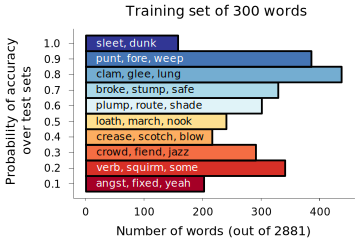
\includegraphics[width=0.9\columnwidth]{figures/word_accuracy_over_testsets.png}

	\caption{When aggregating over the 100k 300-word model training environments, each word occurs in many test sets. The proportion of times a word occurs in the test set and is accurately generalized to corresponds to how difficult that word is to learn. Representative words belonging to each bin are displayed.}
	\label{word_acc_hist}
\end{figure}

At one extreme are words that are accurately generalized to with almost any random selection of words, and at the other are words that can only be accurately generalized to if particular (combinations of) words are present in the training set. This latter set of words has mappings between orthography and phonology that are highly atypical in light of the rest of the corpus, or are comprised of very low frequency combinations of letters, while the former contain spelling patterns and phonological mappings that occur often within the corpus.

Whether a word was likely to be generalized to was related to quantifiable measures of orthographic, phonological, and relational typicality.
% For each word, we computed the mean pairwise distance between its orthographic representation and the orthographic representations of all other words in the corpus. The same was done for the phonological representations, and representations associated with the mapping between orthography and phonology obtained by training an instance of our model on all words in the corpus until mastery (all phonological outputs are accurate) and extracting the 100 unit hidden layer activation for each word. These will be referred to as the \emph{mapping representations}. Standard deviations (SD) were recorded along with the means of these pairwise distances.
We considered word length, orthographic neighborhood size, phonological neighborhood size, and orth-phon consistency:
\begin{itemize}
	\item A word's length is the number of letters in it's orthography.
	\item A word's orthographic neighborhood is composed of words whose othography is one letter swap, drop, or addition away from being the same ($D_{Levenschtein} < 1$).
	\item A word's phonological neighborhood is composed of words with shared rimes.
	\item A word's consistency was determined by first identifying the set of words that share its ``orthographic body''---the first vowel and all letters following it---and then counting the number of words in that subset which share a rime.
	The consistency metric is the proportion of words that share both an othographic body that also share a phonological rime \cite{Plaut1996}.
\end{itemize}

% WE ENDED UP NOT USING ANYTHING BASED ON THIS REFERENCE MODEL
%We also explored a less conventional metric, derived from representations obtained by training an instance of our model on all words in the corpus until mastery (all phonological outputs are accurate).
%The 100 unit hidden layer activations for each word will be referred to as the \emph{mapping representations}, because they correspond to the model's internal representation of the ``mapping'' between orthography and phonology in our model environment.
%Because they stand between the two modalities, these representations give an alternative insight into consistency that may help address a limitation of conventional consistency metrics.

\begin{table}
	\begin{tabular}{r r r r r}
		                     & WL & ON & PN & Con. \\
       \toprule
		\textit{Word Length}          &  1.00 & & & \\
		\textit{Orth. Neighbors}      & -0.65 &  1.00 & & \\
		\textit{Phon. Neighbors}      & -0.28 &  0.35 &  1.00 & \\
		\textit{Consistency}          & -0.03 & -0.02 & -0.02 & 1.00 \\
		\midrule
		\textit{P(accuracy)}          & -0.27  & 0.47 & 0.28 & 0.38 \\
	\end{tabular}
	\caption{Correlation among variables of interest. The bottom row reports the pairwise correlation of each variable with the probability of generalization accuracy for each word, defined as the number of times accurately generalized to divided by the number of test sets a word appeared in.} 
	\label{tab:cormat}
\end{table}

%
%\begin{figure}[t]
%	\includegraphics[width=0.9\columnwidth]{figures/word_accuracy_by_hiddenSD.png}
%	
%	\caption{The probability of accurate generalization to each word, regressed on the standard deviation (SD) of the distance between each word's ``mapping'' representation and the mapping representations of other words, after removing variance explained by mean orthographic and phonological distance. This metric will be low for words that have a high mean distance while utilizing dimensions in the representational space that are relatively unused by other words.}
%	\label{word_acc_regression}
%\end{figure}

\begin{table}[b]
	\begin{center}
		\begin{tabular}{r r r r r}
			\textbf{regressor} & $\eta^2_p$ & $\Delta \mathbf{R^2}$ \\
			\toprule
\textit{Word length}       & 0.01 & 0.00 \\
\textit{Orth. Neighbors}   & 0.17 & 0.13 \\
\textit{Phon. Neighbors}   & 0.03 & 0.02 \\
\textit{Consistency}       & 0.20 & 0.15 \\
\bottomrule

		\end{tabular}
		\caption{Effect sizes for the regressors used to account for variance in the probability of accurately generalizing each word. These effect size metrics are perspectives on the unique variance explained by each variable. Because of collinearity among the regressors, the sum of the $\Delta R^2$ values will be less than total $R^2 = 0.39$.}
		\label{tab:effectsize}
	\end{center}
\end{table}

The correlations among these variables, and between these variables and the probability of accurate generalization, are reported in Table \ref{tab:cormat}.
The number of orthographic neighbors tends to decrease as word length increases (r = -0.65); a similar but weaker trend applies to the size of phonological neighborhoods (r = -0.28).
This is representative of the English language in general.
There is also a moderate relationship between neighborhood size across modalities, such that words that belong to large othographic neighborhoods are expected to belong to large phonological neighborhoods (r = 0.35).
That this correlation is not higher demonstrates the asymmetry of structure across the modalities.
The consistency of a word's pronunciation given its orthography, however, is uncorrelated with the modality-specific metrics.
Words are more likely to be generalized to if they are short, belong to large phonological and (especially) orthographic neighborhoods, and have consistent pronunciation given their spelling (Table \ref{tab:cormat}, bottom row).
%This is consistent with previous work that focused on performance \cite{Jared1990} and learning \cite{Plaut1996} showing that consistent words and phonotactically probable words \cite{Storkel2003} are easier to incorporate into the vocabulary than inconsistent ones.

Given the high correlations among variables, and to gain perspective on how jointly-predictive these factors are of the probability of accurate generalization, we regressed the probability of accuracy over test sets on all four variables in an additive linear model (no interaction terms).
This simple model accounts for only 39\% of the variance in generalization accuracy.
Of the variables we considered, the consistency metric accounted for the most unique variance ($\Delta R^2 = 0.15$), but orthographic neighborhood size was a close second ($\Delta R^2 = 0.13$). Once accounting for other variables, phonological neighborhood size and word length did not appreciably improve the model.

It is important to note that the focus on spelling-sound consistency is indeed not novel, but important in the context of understanding generalization. Consistency effects in word reading have been demonstrated in performance \cite{Jared1990,Plaut1996} and learning \cite{Seidenberg1989}, while our study emphasizes this important component of cross-modal learning in reading specifically in the context of patterns of generalization emergent from models learning in different environments.

%While we 
Out of the variables we considered, phonological neighborhood size is the most studied in the context of word acquisition, where it is understood to influence the order in which words are acquired \cite{Storkel2003}.
Orthographic neighborhood size is often studied in terms of performance, specifically visual word recognition and lexical access \cite{Andrews1997}.
It is also negatively correlated with age of acquisition norms, which indicates that words with more dense orthographic neighborhoods tend to be learned earlier \cite{Cameirao2010}.
Words with consistent orthographic to phonology relationships are also processed more efficiently \cite{Ziegler2004}.

\subsection{What makes a good training set?}
The word-level features reviewed above give some insight into which words will tend to be generalized to, and which will not, in the context of any given training set.
The deeper question regards what qualities of the training set will foster the most generalization to untrained words in the language.
One angle on this question is to consider that the word-level features are in fact reflective of how the word is situated relative to the broader linguistic environment.
While we did not test this directly, it is plausible to assume that neighborhood size predicts how likely a word is to be generalized to.
Good training sets are \textit{representative} of the broader environment.
If a neighborhood is split across training and test sets, the consequence is that the neighbors in the test set have representation within the training set.
Given that we randomly split our corpus into training and test sets, there is no guarantee that neighborhoods are efficiently split in this way.
However, words that belong to larger neighborhoods are more likely to be split across training and test sets by chance, so we might expect that training sets with larger orthographic and phonological neighborhoods on average will be foster more generalization.
It is clear that words with no orthographic neighbors (n=271) are generalized to far less often (median probability 0.10) than words with at least one neighbor (median probability 0.56).

Such a crude metric, however, would be largely insensitive to relative composition of the two sets.
For instance, training sets that contain many words with large neighborhoods may simply contain all the words belonging to those large neighborhoods.
Such a training set would be very unrepresentative of the test set, and unlikely to foster generalization.
What we would rather know is each word's neighborhood size and relative to the number of its neighbors that also belong to the training set.

On the other hand, orthographic and phonological neighborhood structure is only helpful to the extent that they are aligned.
An orthographic neighborhood populated with words with irregular and idiosyncratic pronunciations is not likely to foster generalization on a reading-aloud task.
Thus, training sets that have a large and varied collection of words with consistent pronunciations may be expected to generalize well.
While it is easy to determine the mean consistency of a training set, it is less clear how to account for the variability across consistent relationships.
%These are avenues of metric development that will be critical for understanding the 

As an initial attempt, we regressed the generalization preformance of the 100,000 models trained on 300 word training sets on the mean word length, orthographic and phonological neighborhood sizes, and consistency over all 300 words in each set.
The effect sizes are reported in Table \ref{tab:effectsize_model}.
We see that, despite being a very crude measure, mean orth-phon consistency accounts for about 13.6\% of the variance unexplained by the other variables, indicating that item level characteristics may provide insight on how to construct efficient training sets.
However, the vast majority of variance remains unexplained and provides fertile ground for continued research.

\begin{table}
	\begin{center}
	\begin{tabular}{r r r}
					\textbf{regressor} & $\eta^2_p$ & $\Delta \mathbf{R^2}$ \\
		\toprule
		\textit{Word length}       & 0.002 & 0.001 \\
		\textit{Orth. Neighbors}   & 0.006 & 0.005 \\
		\textit{Phon. Neighbors}   & 0.000 & 0.000 \\
		\textit{Consistency}       & 0.137 & 0.136 \\
		\bottomrule
		
	\end{tabular}
\end{center}
\caption{Effect sizes for the regressors used to account for variance in generalization accuracy over the 100,000 models fit to random 300 word training sets. Generalization was to all untrained words in the corpus. Because of collinearity among the regressors, the sum of the $\Delta R^2$ values will be less than total $R^2 = 0.14$.}
\label{tab:effectsize_model}
\end{table}



%The SD of the distances to a point emphasizes its position within the coordinate space in a way that is quite different from the mean. Consider a set of points that fall on a line. If we take one of those points and move it along the line, its mean distance from the other points will change \emph{but the SD of the distances will not}. Now, if we take that same point and pull it off the line, into a second dimension, the mean distance will grow as the point continues its excursion in the new dimension. \emph{The SD among those distances, however, will shrink}. In other words, words with small SDs are likely to occupy idiosyncratic ``representational niches''. We would expect ``sight words'' to occupy such niches, and indeed words like \exword{quay} (pronounced ``key'') and \exword{queue} (pronounced ``cue'') have the lowest SD. Quay in particular has the \nth{2} smallest SD and the \nth{2045} largest mean over distances to the other words; the SD is consistent with its atypicality, while the mean misrepresents it as being very similar to other mappings.
%
%Regressing the probability of accurate generalization for each word on its mean orthographic distance, mean phonological distance, and the SD of distances to mapping representations accounts for 22\% of the overall variance in generalization error, with mapping representation SD metric accounting for about 10\% of the variance. Table 2 reports the effect size of each regressor, emphasizing the relative importance of the SD variable. Figure \ref{word_acc_regression} displays the model plotted over the accuracy data for each word, with variance explained by orthographic and phonological mean distance removed, while orthographic and phonological mean distance are held constant at their means.


\section{Discussion}
We have established a computational procedure for investigating two aspects of generalization in learning basic reading skills: how many words need to be learned to generalize to real English words yet to be learned, and what aspects of reading vocabulary promote this transfer.  Our findings indicate that while printed vocabulary continues to grow along the number of words taught, the efficiency of learning does not grow along with it.

As the teacher grows the number of words they would like to teach, the amount of learning time needed grows along with it. Our findings suggest a trade-off where a smaller number of words could be taught, optimizing efficiency of learning and teaching for sake of near-optimal generalization capacity. This has substantial implications for reading education where very often exhaustive sequential instruction of rule-based mappings from print to sound dominate in pedagogical approaches that consider phonics skills valuable to students. This approach could be particularly useful for students that need to catch up due to insufficient reading skills. When learning to read is cast as a generalization problem we may more easily be able to help students that require the most care and attention, where time is of the essence, by targeting specific deficits in her or his capacity to generalize knowledge to the printed language.

The problem of maximizing generalization with the smallest possible training set can be formalized as a \emph{machine teaching} optimization problem \cite{Zhu2015}. We have drawn on this literature by manipulating the learning environment while holding the abilities of the learner constant, and then performing careful analyses of the outcomes to identify the factors that contribute to training the most proficient models. In doing so we have demonstrated systematic relationships between the composition of the training set and generalization performance that machine teachers may be able to discover and exploit. 

These results are empirical; our next step will be to identify properties of words and word-sets responsible for better generalization both at the word- and set-level. As indicated in our regression model reported, item-wise measures of phonology, orthography, and especially the mapping representation account for non-trivial amounts of generalization error. Next steps will be oriented towards accounting for more of the variance in generalization accuracy, and to scale up analyses to model-wise characteristics that promote generalization. It may also be possible to improve efficiency even further by using training sets attuned to children's vocabulary development, and by optimizing the sequence of learning experiences.

Though preliminary, these simulations demonstrate that it is possible to be more efficient with curricula that attend to the number of words taught and the words that are prioritized in teaching.

%\section{Acknowledgments}
%The research reported here was supported by the Institute of Education Sciences, US Department of Education, through Award \#R305B150003 to the University of Wisconsin, Madison. The opinions expressed here are those only of the authors and do not at all represent the views of the U.S. Department of Education. The Center for High Throughput Computing (CHTC) is supported by UW-Madison, the Advanced Computing Initiative, the Wisconsin Alumni Research Foundation, the Wisconsin Institutes for Discovery, and the National Science Foundation, and is an active member of the Open Science Grid, which is supported by the National Science Foundation and the U.S. Department of Energy's Office of Science.


\bibliographystyle{apacite}

\setlength{\bibleftmargin}{.125in}
\setlength{\bibindent}{-\bibleftmargin}

\bibliography{CogSci_2019_CoxCooperBorkenhagenSeidenberg}


\end{document}
